%\documentclass[a4paper,12pt,titlepage]{article}
\documentclass[10pt]{article}
\title{COMP4490 - Computer Graphics 2 \\ Project Report \\ Investigation of Non-Photorealistic Filters and their Effects on Images and Video}
\author{Robin Swanson \& Nico Richard\\ umswans5@myumanitoba.ca umrich84@myumanitoba.ca}
\date{April 2014}
\usepackage{hyperref}
\usepackage{graphicx}
\usepackage{parskip}
\usepackage{mathtools}
\usepackage{caption}
\usepackage{subcaption}
\usepackage{array}
\usepackage{fancyhdr}
\pagestyle{fancy}
\usepackage[margin=1in]{geometry}
\fancyhead[R]{Robin Swanson \& Nico Richard - Project Report}
\begin{document}
\maketitle

For our project we implemented various non-photo-realistic image filters resulting in a "cartoon-ish" effect. We were also able to implement a rudimentary pipeline for splitting an input video into frames, applying a filter to each frame, and recombining them. This was accomplished using the ffmpeg toolset as well as the OpenMP library to parallelize the operations.

Here we include some example output from the various filters we were able to implement as well as any additional details pertinent to their implementation.

Examples of output \footnote{Long DoGs -- \url{https://www.youtube.com/watch?v=jtmSWE7YlcA}} videos\footnote{Short DoGs -- \url{https://www.youtube.com/watch?v=yUu6u1vjXO4}} can be found on our YouTube account.

All source code can be found on our Github\footnote{Soderberg on GitHub -- \url{https://github.com/CityTransit/Soderberg}}.

\section{Filter Details}

\begin{itemize}

\item Bilateral Filter: The Bilateral Filter is a simple gaussian (spacial, pixel value, and temporal) convolution. Smooths colours similar to a gaussian blur while preserving edge values. Currently implemented and working correctly.

\item Kuwahara Filter: This filter explores regions nearby to the pixel and chooses the RGB value of the area with the smallest deviation of colour. Currently implemented and working correctly.

\item Anisotropic Kuwahara Filter: Similar to the standard Kuwahara filter, but aims to preserve directionality of colour by modifying the regions explored based on a smoothed structure tensor. Currently implemented but \emph{not} working correctly.

\item Difference of Gaussian Filter: By convolving the image with two Gaussian kernels of different sizes we can take the difference of the two and use it as a band bass filter. This allows us to approximate the Laplacian of Gaussian equation. When the size of the second kernel is approximately 1.6 times the size of the first we can use the result as a cartoon-like effect. Currently implemented and working correctly.

\item eXtended Difference of Gaussian Filter: By extending the standard Difference of Gaussian filter with a threshold function with a continuous ramp we can improve noise reduction and appearance. I've also done some re-parametrization of the filter to allow for strong customization. Currently implemented and working correctly.

\item Utility Filters: A Gaussian Filter for blurring and a Sharpening Filter to increase the definition of edges as well as a Kernel class capable of generating classical sobel, box blurring, and more! Currently implemented and working correctly.
\end{itemize}


\begin{figure}
\centering
\begin{subfigure}[b]{0.45\textwidth}
	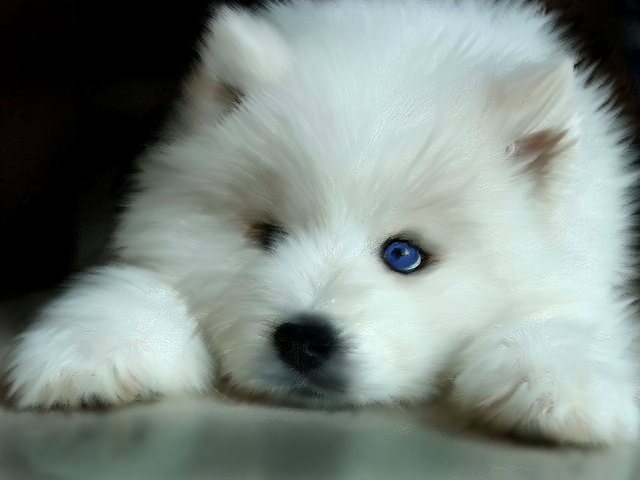
\includegraphics[width=\textwidth]{test_image}
	\caption{Our test input image before any modifications have been made.}
\end{subfigure}
\begin{subfigure}[b]{0.45\textwidth}
	\includegraphics[width=\textwidth]{test_out_bilat}
	\caption{Test input image modified using the Bilateral Filter.}
\end{subfigure}
\begin{subfigure}[b]{0.45\textwidth}
	\includegraphics[width=\textwidth]{test_out_kuwa}
	\caption{Test input image modified using the Kuwahara Filter.}
\end{subfigure}
\end{figure}

\begin{figure}
\centering
\begin{subfigure}[b]{0.45\textwidth}
	\includegraphics[width=\textwidth]{Lenna}
	\caption{Our test input image before any modifications have been made.}
\end{subfigure}
\begin{subfigure}[b]{0.45\textwidth}
	\includegraphics[width=\textwidth]{applyDoG}
	\caption{Test input image modified using only the Difference of Gaussian Filter.}
\end{subfigure}
\begin{subfigure}[b]{0.45\textwidth}
	\includegraphics[width=\textwidth]{applyColorXDoG}
	\caption{Test input image modified using the XDoG Filter with added colour.}
\end{subfigure}
\end{figure}

\section{Implementation Details}

All of the code found in our work is original work written by us based on the reference papers with only two exceptions:

\begin{itemize}
\item The libpng code to read and write .png files was largely based on example code from libpng sources as there was no significant need or reason to write our own implementation. However, they were modified to suit our needs (e.g., removal of alpha channels, etc.).

\item The current state of the Anisotropic Kuwahara filter (at the moment not working properly) is largely based on a GLSL implementation\footnote{polyakf on Google Code -- \url{http://code.google.com/p/polyakf/}} in an effort to debug the filter and much of our original implementation was lost at some point. This filter proved to be quite difficult to implement, and continues to elude us. The principles behind it are fairly easy to understand, but modifying the circular search regions was a more interesting problem than anticipated. As it currently stands, the filter in no way affects the output image.
\end{itemize}


\section{Using The Code}
We've included a simple make file to make compilation somewhat easier. The simplest way to get up and running may be to clone the git repo on Aviary and use the Aviary make flag.

\begin{verbatim}
git clone https://github.com/CityTransit/Soderberg.git
make aviary
\end{verbatim}

We've also included a sample main file (batch.cpp) which uses OpenMP to provide some high level parallelism. This file can be used as a sample to create your own programs or modified to test different filters.

\section{Future Work}
Fixing the Anisotropic Kuwahara filter, obviously, would have been ideal. Unfortunately it proved to be quite difficult to implement.

More fine-grained parallelism would have been nice to exploit. Image filters are inherently embarrassingly parallel and it would not have been too difficult to implement. However, for this project we were much more interested in exploring a breadth of filters than perfecting any one filter.

\begin{thebibliography}{99} % 

\bibitem{bilateral}
Tomasi, C., Manduchi, R.: Bilateral filtering for gray and color images. In: Proc. ICCV, pp. 839–846 (1998). doi: 10.1109/ICCV.1998.710815

\bibitem{AKF}
Kyprianidis, J.E., Kang, H., Döllner, J.: Image and video abstraction by anisotropic Kuwahara filtering. Comput. Graph. Forum 28 (7), 1955–1963 (2009). doi:10.1111/j.1467-8659.2009.01574.x

\bibitem{dog}
Winnemöller, H., Kyprianidis, J.E., Olsen, S.C.: XDoG: an extended difference-of-Gaussians compendium including advanced image stylization. Comput. Graph. 36 (6), 740–753 (2012). doi:10.1016/j.cag.2012.03.004

\bibitem{fbdog}
Kang, H., Lee, S., Chui, C.K.: Flow-based image abstraction. IEEE Trans. Vis. Comput. Graph. 15 (1), 62–76 (2009). doi: 10.1109/TVCG.2008.81

\bibitem{moredog}
Kyprianidis, J.E., Döllner, J.: Image abstraction by structure adaptive filtering. In: Proc. EG UK TPCG, pp. 51–58 (2008). doi: 10.2312/LocalChapterEvents/TPCG/TPCG08/051-058

\bibitem{weickert}
Torre, V., Poggio, T.A.: On edge detection. IEEE Trans. Pattern Anal. Mach. Intell. 8 (2), 147–163 (1986). doi: 10.1109/TPAMI.1986.4767769

\bibitem{book}
"Image and Video-Based Artistic Stylisation"; Paul Rosin, John Collomosse; Computational Imaging and Vision, Volume 42 (2013)


\end{thebibliography}
\end{document}
